\chapter{Swaps and Bootstrapping}\label{sec:swaps-and-bootstrapping}

In this Chapter the Overnight Index Swap contract is reviewed and a class to represent it will be added to our financial module. Beside financial arguments another very important mathematical technique is introduced: the \emph{bootstrapping}.

\section{Payment Dates Generator}
Before going to describe the Overnight Index Swap we need to develop a tool which helps us to generate list of dates (e.g. payment dates), a task that we need to do often from now on. 
The function we are writing will go in \texttt{finmarkets} module and will be used by the classes describing various kind of contracts.

\begin{ipython}
from datetime import date
from dateutil.relativedelta import relativedelta

def generate_dates(start_date, n_months):
    dates = []
    for i in range(0, n_months, 12):
        dates.append(start_date + relativedelta(months=i))
    dates.append(start_date + relativedelta(months=n_months))
    return dates

print (generate_dates(date.today(), 25))
\end{ipython}
\begin{ioutput}
[datetime.date(2020, 10, 20), datetime.date(2021, 10, 20), datetime.date(2022,
10, 20), datetime.date(2022, 11, 20)]
\end{ioutput}

\begin{finmarkets}
Add this utility function in \texttt{finmarkets.py} since it will be used very often later on.
\end{finmarkets}

\section{Overnight Index Swap}\label{overnight-index-swap}

Interest rate swaps (IRS) are generally used to mitigate the risks of fluctuations of varying interest rates, or to benefit from lower rates.

Overnight Index Swaps (OIS) are a particular kind of IRS which pay a floating coupon, determined by overnight rate fixings over the reference periods, against a fixed coupon. By definition an OIS is defined by:

\begin{itemize}
\tightlist
\item
  a notional amount \(N\);
\item
  a starting date \(d_0\);
\item
  a sequence of payment dates \(d_1,...,d_n\);
\item
  a fixed rate \(K\).
\end{itemize}

For simplicity in the following we are assuming that the fixed and floating legs of our OIS have the same notional and payment dates, although this is not necessarily always the case in practice. We will always look at these products from the point of view of the \textbf{receiver of the floating leg}.

\subsection{OIS Valuation}\label{ois-valuation}
To evaluate the net present value (NPV) of such products the cash flows of each leg have to be calculated; today's NPV then is the sum of all the discounted cash flows.

\subsubsection{Floating leg}\label{floating-leg}

At each payment date, the floating leg pays a cash flow determined as follows:

\begin{equation}
f_{\mathrm{float},~i} = N \Bigg\{\prod_{d=d_{i-1}}^{d=d_i-1}\Big(1+r_{\mathrm{O/N}}(d)\cdot\frac{1}{360}\Big) -1 \Bigg\}
\label{eq:floating_ois}
\end{equation}

Strictly speaking this formula is valid for an EONIA swaps (i.e. for OIS swaps in EUR) other currencies might have different conventions. The \(\frac{1}{360}\) fraction appears because EONIA rates are quoted using the ACT/360 day-count convention. In addition we are making the simplifying assumption of ignoring weekends and holidays, so we assume that each overnight rate is valid for only one day. The sum of the discounted expected values of these cash flows is

\begin{equation}
\mathrm{NPV}_{\mathrm{float}} = \sum_{i=1}^{n}D(d_i)\mathbb{E}[f_{\mathrm{float},~i}]
\end{equation}
where \(D(d)\) is the discount factor with expiry \(d\). On the other hand we have seen from the forward rate definition (see Section~\ref{calculating-forward-rates}) that

\begin{equation*}
\prod_{i=0}^{d} (1+r_i) = \underbrace{(1+r_{0,1}\Delta T)\underbrace{(1+r_{1,2}\Delta T)\ldots\underbrace{(1+r_{d-2,d-1}\Delta T)(1+r_{d-1,d}\Delta T)}_{=(1+r_{d-2,d}\Delta T)}}_{=(1+r_{1,d}\Delta T)}}_{=(1+r_{0,d}\Delta T)}
\end{equation*}
So Eq.~\ref{eq:floating_ois} can be simplified into

\begin{equation}
\mathbb{E}[f_{\mathrm{float},~i}] = N\cdot\Big(\frac{D_{\mathrm{OIS}}(d_{i-1})}{D_{\mathrm{OIS}}(d_{i})} - 1\Big)
\end{equation}
hence
\begin{equation}
\mathrm{NPV}_{\mathrm{float}} = N\cdot \sum_{i=1}^{n}D(d_i) \Big(\frac{D_{\mathrm{OIS}}(d_{i-1})}{D_{\mathrm{OIS}}(d_{i})} - 1\Big)
\end{equation}
where \(D_{\mathrm{OIS}}(d)\) is the discount factor implied by OIS prices (we will see how to derive it).

%The correct curve to use for discounting the flows of a collateralized contract, like OIS, is the one associated with the collateral. Since OIS contracts are collateralized with cash, and cash accrues daily interest at the overnight rate, the OIS curve is itself the correct curve with which to discount the flows of an OIS contract ! 
%From what has been said in Section~\ref{sec:financial-crisis}
%Since the financial crisis, in the Euro area the rates used for
%discounting has been the EONIA rates. Similarly, in other jurisdictions
%it has been used other overnight rates such us Fed fund rates in USA.
%This practice is consistent with the daily remuneration of the
%collateral (i.e. cash given or received as mitigants for credit risk
%arising from the mark to market of the derivatives contract).
%For arbitrage consideration the discounting curve of future cash flows
%in a derivative contract can only be the one derived from the rates
%applied for the collateral.
%
%So we have that \(D = D_{\mathrm{OIS}}\) and the NPV simplifies to

From what has been said in Section~\ref{sec:financial-crisis} we have that \(D = D_{\mathrm{OIS}}\) and the NPV simplifies to

\begin{equation}
  \begin{split}
    \mathrm{NPV}_{\mathrm{float}} & = N\cdot\sum_{i=1}^{n}[D(d_{i-1}) - D(d_i)] =  \\
    &= N\cdot[(D(d_{0}) - D(d_{1})) + (D(d_{1}) - D(d_{2})) + ... + (D(d_{n-1}) - D(d_{n}))]\\
    &= N \cdot [D(d_0) - D(d_n)]
  \end{split}
\end{equation}

\subsubsection{Fixed leg}\label{fixed-leg}

The calculation for the fixed leg is simpler; each cash flow is equal to

\begin{equation}
f_{\mathrm{fixed},~i}=N\cdot K\cdot \frac{d_i - d_{i-1}}{360}
\end{equation}
so the NPV of the fixed leg is

\begin{equation}
\mathrm{NPV}_{\mathrm{fixed}} = N\cdot K\cdot \sum_{i=1}^{n}D(d_{i})\frac{d_i - d_{i-1}}{360}
\end{equation}

\subsection{\texttt{OvernightIndexSwap} Class}\label{discount-factor-determination-from-market-quotes}

\textbf{Our ultimate goal is to take a series of Overnight Index Swap quotations, and determine the discount factors implied by their prices.} To do this we will build a class to represent OIS and compute its value, given a particular discount curve. Then we will use this class, put inside a numerical optimizer, to \emph{invert} the relationship that connects NPV and discount curve so that the \emph{implied} discount factors can be determined from OIS market quotes.

The \texttt{OvernightIndexSwap} class will have also a method called \texttt{fair\_value\_strike} which takes a discount curve object and returns the fixed rate which would make the OIS net present value (NPV) zero. This is quite easy since it is enough to equal the expressions for the NPV of each swap leg and solve for $K$.

\begin{equation}
\begin{gathered}
K \sum_{i=1}^{n}D(d_{i})\cfrac{d_i - d_{i-1}}{360} = [D(d_0) - D(d_n)] \\
K = \cfrac{[D(d_0) - D(d_n)]}{\sum_{i=1}^{n}D(d_{i})\cfrac{d_i - d_{i-1}}{360}}
\end{gathered}
\end{equation}

\begin{ipython}
class OvernightIndexSwap:
    def __init__(self, notional, payment_dates, fixed_rate):
        self.notional = notional 
        self.payment_dates = payment_dates
        self.fixed_rate = fixed_rate

    def npv_floating_leg(self, discount_curve):
        return self.notional * (discount_curve.df(self.payment_dates[0]) -
                                discount_curve.df(self.payment_dates[-1]))

    def npv_fixed_leg(self, discount_curve):
        npv = 0
        for i in range(1, len(self.payment_dates)):
            start_date = self.payment_dates[i-1]
            end_date = self.payment_dates[i]
            tau = (end_date - start_date).days / 360
            df = discount_curve.df(end_date)
            npv = npv + df * tau
        return self.notional * self.fixed_rate * npv

    def npv(self, discount_curve):
        float_npv = self.npv_floating_leg(discount_curve)
        fixed_npv = self.npv_fixed_leg(discount_curve)
        return float_npv - fixed_npv

    def fair_value_strike(self, discount_curve):
        den = 0
        for i in range(1, len(self.payment_dates)):
            start_date = self.payment_dates[i-1]
            end_date = self.payment_dates[i]
            tau = (end_date - start_date).days / 360
            df = discount_curve.df(end_date)
            den += df * tau
            num = (discount_curve.df(self.payment_dates[0]) -
                discount_curve.df(self.payment_dates[-1]))
        return num/den

\end{ipython}

\begin{finmarkets}
This class also goes into \texttt{finmarkets.py} library as a useful tool to work with Overnight Index Swaps.
\end{finmarkets}

To test it a discount curve is needed. In the following example a fake curve is defined and used with an OIS product.

\begin{ipython}
from datetime import date
from finmarkets import DiscountCurve

ois = OvernightIndexSwap(# the notional, one million
                         1e6,
                         # the list of product dates,
                         # i.e. the start date then the payment dates
                         [date(2020, 1, 1), date(2020, 4, 1),
                          date(2020, 7, 1), date(2020, 10, 1),
                          date(2021, 1, 1)],
                         # the fixed rate, 2.5%
                         0.025)

curve = DiscountCurve([date(2020, 1, 1), date(2021, 6, 1),
                       date(2022, 1, 1)],
                      [1.0, 0.98, 0.82])

print ("OIS NPV : {:.2f}".format(ois.npv(curve)))
\end{ipython}
\begin{ioutput}
105332.19
\end{ioutput}

\section{Bootstrap Technique}
\label{bootstrapping-technique}

As we said before we would like to determine a \emph{real} discount
curve starting from the market quotes of a set of Overnight Index Swaps with different maturities. This will be done via a technique called bootstrapping which is the abc of financial mathematics, since a discount curve to price a contract is always needed.

We are going to concentrate on EONIA swaps in order to build an EUR discount curve.

\subsection{Building OIS Instances}
\label{building-ois-instances}

The first step involves getting data, the swap market quotes, and this is not actually as simple as it sounds.

The issue is that EONIA swap market is over the counter (OTC) and it's not straightforward to access it. Unlike (some) listed futures, where anyone with a retail brokerage account can view and apply real time prices, to trade in the EONIA swap market you have to be a financial institution or at least a large company and have an agreement with a broker which operates in the market. One of the most important broker in the OIS market is ICAP, see Fig.~\ref{fig:icap}.

\begin{figure}[bth]
  \centering
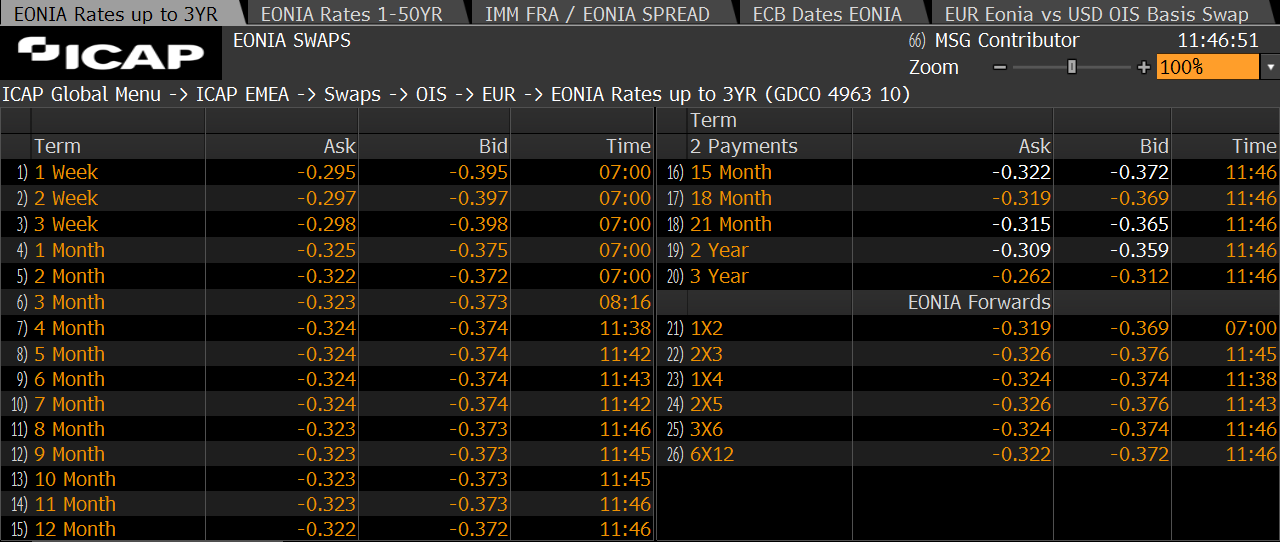
\includegraphics[width=1.\linewidth]{figures/icap_3.png}
\caption{Screenshot of market quotes from ICAP.}
\label{fig:icap}
\end{figure}

Though there exist some electronic platform in which market participants post bids and offers and other participants can apply them, in practice a lot of trading is still done over "voice", i.e.~by phone or more commonly over chat. For convenience, however, Bloomberg provides a service which displays indicative real time rates as provided by a selection of relevant brokers. Note that interest rate swap quotes vary from standard price quotes of commonly traded instruments, they can appear puzzling but the quotes are effectively interest rates.

In the following we use a manually created dataset (\href{https://github.com/matteosan1/finance_course/raw/develop/libro/input_files/ois_data.xlsx'}{\texttt{ois\_data.xlsx}}) to derive the discount curve. With the help of \texttt{pandas} the dataset can be inspected:

\begin{ipython}
import pandas as pd
from datetime import date

observation_date = date.today()
mq = pd.read_csv('https://github.com/matteosan1/finance_course/raw/develop/libro/input_files/ois_data.xlsx')
print (mq.head())
\end{ipython}
\begin{ioutput}
   months  quote
0       1 -0.350
1       2 -0.347
2       3 -0.348
3       4 -0.350
4       5 -0.350
\end{ioutput}

Let's say we want to build a 15 months swap instance using data contained in \texttt{ois\_data.xls}. Be careful when doing this
operation and double check the units of rates and quotes. In this case for example quotes are expressed in percent so you need to multiply by 0.01 to use them. Another misleading detail to check is the correct index of a particular quote. For example the 15 months quote is not the fifteenth entry in the dataframe but rather the twelfth.

\begin{ipython}
ois = OvernightIndexSwap(1e6,
                         generate_dates(date.today(), 15),
                         mq.loc[mq['months']==15, 'quote']*0.01)

ois.payment_dates[-1]
\end{ipython}
\begin{ioutput}
datetime.date(2023, 1, 1)
\end{ioutput}

To use the \texttt{npv} method, to calculate the OIS's NPV, we need a discount curve and here comes to hand the bootstrapping technique !

\subsection{Constructing the Yield Curve}
\label{the-bootstrapping-technique}

Let's keep aside for a moment our swaps and introduce the \emph{bootstrap algorithm}. In finance, bootstrapping is a method for constructing a yield curve from the prices of a set of coupon-bearing products, e.g. bonds and swaps. The term structure of spot returns is obtained from the product yields by solving for them recursively, by forward substitution: this iterative process is what is called the bootstrap method. 

The usefulness of bootstrap resides on that using only a few carefully selected products, it is possible to derive forward and spot rates for all maturities, i.e. given the solved curve.

This algorithm relies on the assumption that market quotes represent the \textbf{fair price} of the contracts so they make their NPVs null (the fair price is an estimate of what a willing buyer would pay a willing seller for a given asset, assuming both have a reasonable knowledge of the asset's worth).

To illustrate bootstrapping let's consider the following example: we have some coupon paying bond (coupon of 4\%, 5\%, 6\%, 7\% and 8\% respectively) with maturities ranging from 1 to 5 years, each having a value of \euro{100} and traded at par. To determine the yield curve proceed as follows:
\begin{enumerate}
\item at the end of the first year the $1^{st}$ bond will pay a coupon of \euro{4} (= \euro{100} * 4\%) plus the principal (= \euro{100}) which sums up to \euro{104} while the bond is trading at \euro{100}. The implied 1-year spot \emph{fair} rate $S_{1y}$ can be calculated from $\mbox{\euro{100}} = \mbox{\euro{104}} / (1 + S_{1y})$;

\item at the end of second year the sum of the cash flows of the $2^{nd}$ bond can be compared to its trading price to compute the 2-year spot rate $S_{2y}$ from $\mbox{\euro{100}} = \mbox{\euro{5}} / (1 + S_{1y}) + \mbox{\euro{105}} / (1 + S_{2y})^{2}$ where the previously derived value of $S_{1y}$ is used;

\item at the end of third year the sum of the cash flows of the $3^{rd}$ bond can be compared to its trading price to calculate the 3-year spot rate $S_{3y}$ as $\mbox{\euro{100}} = \mbox{\euro{6}} / (1 + S_{1y}) + \mbox{\euro{6}} / (1 + S_{2y})^{2} + \mbox{\euro{106}} / (1 + S_{3y})^{3}$, using $S_{1y}$ and $S_{2y}$ computed before;

\item and so on for all the other bonds\ldots
\end{enumerate}

Putting all together we can construct a system of equations (now omitting the currency symbol for simplicity):

\begin{equation}
\begin{cases}
100 = \cfrac{104}{(1 + S_{1y})} \\
100 = \cfrac{5}{(1 + S_{1y})} + \cfrac{105}{(1 + S_{2y})^{2}} \\
100 = \cfrac{6} {(1 + S_{1y})} + \cfrac{6}{(1 + S_{2y})^{2}} + \cfrac{106} {(1 + S_{3y})^{3}} \\
100 = \cfrac{7} {(1 + S_{1y})} + \cfrac{7} {(1 + S_{2y})^{2}} + \cfrac{7} {(1 + S_{3y})^{3}} + \cfrac{107} {(1 + S_{4y})^{4}} \\
100 = \cfrac{8} {(1 + S_{1y})} + \cfrac{8} {(1 + S_{2y})^{2}}+ \cfrac{8} {(1 + S_{3y})^{3}} + \cfrac{8} {(1 + S_{4y})^{4}} + \cfrac{108} {(1 + S_{5y})^{5}}
\end{cases}
\label{eq:fifth_year_rate}
\end{equation}

This system can be solved quite easily: $S_{1y}$ can be derived from the first equation, $S_{2y}$ from the second, $S_{3y}$ from the third\ldots So

\begin{equation}
100 = 104 / (1 + S_{1y})\quad\Rightarrow\quad S_{1y} = 104/100 - 1 = 4\%
\end{equation}
Moving to the second equation:
\begin{equation}
\begin{split}
& 100 = 5 / (1 + 0.04) + 105 / (1 + S_{2y})^{2}\quad\Rightarrow\quad S_{2y}^2  + 2 S_{2y}  - 0.103030 = 0 \\
& S_{2y} = - 1 \pm \sqrt{1 + 0.103030} = \begin{cases}\text{\sout{-2.05023}} \\ 0.0502\end{cases}
\end{split}
\end{equation}
where the first solution has been discarded because negative.

This equation can be also solved in \texttt{python} with \texttt{numpy.roots}:
\begin{ipython}
import numpy as np
coeff = [1, 2, -0.103030]
np.roots(coeff)
\end{ipython}
\begin{ioutput}
array([-2.05025235,  0.05025235])
\end{ioutput}

From the third equation on it is not as simple to solve them analytically since it involves third (or more) order equations. Luckily it is possible to solve them numerically.

As an example assume all rates up to the fourth year have been calculated (they are reported in Table~\ref{tab:rates}) and just the last one needs to be determined. The last column of Table~\ref{tab:rates} provides the terms to fill the yield curve.

\begin{table}[htb]
\begin{center}
\begin{tabular}{|c|c|c|c|}
\hline
\textbf{years} & \textbf{coupon rate} & \textbf{bond price} & \textbf{spot rate} \\
\hline
1 & 1.00 \% & \euro{100} & 4.00\% \\
\hline
2 & 2.00 \% & \euro{100} & 5.02\% \\
\hline
3 & 3.00 \% & \euro{100} & 6.08\% \\
\hline
4 & 4.00 \% & \euro{100} & 7.19\% \\
\hline
5 & 5.00 \% & \euro{100} & ??? \\
\hline
\end{tabular}
\end{center}
\caption{Table reporting maturity, coupon, bond price and implied spot rate for the example outlined in the text.}
\label{tab:rates}
\end{table}

To solve the last equation numerically one of the root finding algorithm illustrated in Section~\ref{sec:root_finding} can be used. 
In this case \texttt{scipy.optimize.brentq} is used, it finds zeros of a user-defined function within a validity interval.

In Figure~\ref{fig:fifth_year_rate} the last equation of the system in~\ref{eq:fifth_year_rate} is plotted. It already gives us an idea of the expected result, indeed the rate value which solves the equation is around 0.08.

\begin{figure}[htb]
  \centering
  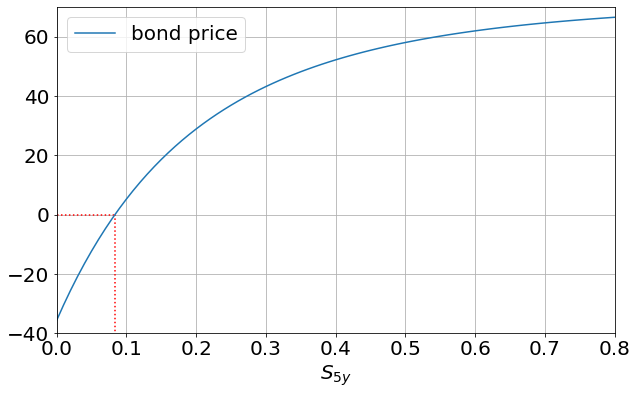
\includegraphics[width=0.7\textwidth]{figures/bond_5_plot.png}
  \caption{Plot of the discounted cash flow of bond 5 as a function of the 5 year spot rate.}
  \label{fig:fifth_year_rate}
\end{figure}

\begin{ipython}
from scipy.optimize import brentq

def func(x):
    return 100 - 8/(1+0.04) - 8/(1+0.0503)**2 - 8/(1+0.0608)**3
               - 8/(1+0.0719)**4 - 108/(1+x)**5
               
a = brentq(func, 0, 0.10)
print ("5y rate: {:.4f}".format(a))
\end{ipython}
\begin{ioutput}
5y rate: 0.0836
\end{ioutput}

The very same mechanism can be generalized and extended to other maturities to get a more detailed yield curve. In general terms the previous system becomes

\begin{equation}
\begin{cases}
f_1(S_1, p_1) = 0 \\
f_2(S_1, S_2, p_2) = 0 \\
f_3(S_1, S_2, S_3, p_3) = 0 \\
f_4(S_1, S_2, S_3, S_4, p_4) = 0 \\
\cdots
\end{cases}
\end{equation}
where $S_i$ are the unknown spot rates and $p_i$ the market quotes of the considered products. The iterative procedure we have applied before exploits the first equation to find $S_1 = f_1^{-1}(p_1)$, the second to find $S_2 = f_2^{-1}(S_1, p_2)$ and so on and so forth. Each equation determines exactly one spot rate which is not already determined by the others.

\subsection{Bootstrapping as Minimization Problem}
\label{sec:bootstrap_as_minimization}
The bootstrap algorithm can now be described in general terms as follows:
\begin{enumerate}
\item define a set of yielding products (e.g. coupon-bearing bonds, swaps\ldots);
%\item derive discount factors for the corresponding terms;
\item \emph{bootstrap} the yield curve, successively calibrating it, such that it returns the input product market quotes.
\end{enumerate}

An alternative way of implementing the bootstrapping, which doesn't relies on  iteratively finding the solution of each equation as before, is to define a vector of spot rates $\mathbf{S} = (S_1, S_2, S_3, \ldots)$ seeking for a particular $\mathbf{\hat{S}}$ which solves the following equation:

\begin{equation}
F = f_1^2(\hat{S}_1,p_1) + f_2^2(\hat{S}_1, \hat{S}_2,p_2) + f_3^2(\hat{S}_1, \hat{S}_2, \hat{S}_3,p_3) + f_4^2(\hat{S}_1, \hat{S}_2, \hat{S}_3, \hat{S}_4,p_4) + \ldots = 0
\label{eq:bootstrap_as_minimization}
\end{equation}

Under this terms the bootstrap method can be considered as a \emph{minimization problem}. In fact we need to find $\mathbf{\hat{S}}$ which \emph{minimize} $F$, (i.e. makes it as close as possible to 0).
Notice how each \(f_i\) is squared since we want all of them to be minimized at the same time and not only \(F\) globally (i.e. without the square there may be cancellation effects between the terms of the sum, which makes $F$ zero but not all $f_i$ individually).

Before implementing the bootstrap method as described let's review the minimization algorithm in general.

\subsection{Minimization Algorithm}
\label{minimization-algorithm}

A minimization algorithm follows these steps:

\begin{itemize}
\tightlist
\item
  define an \emph{objective function} i.e. the function that has to be minimized;
\item
  set the initial value of the unknown parameters (\(\mathbf{x_0}\)) and their range of variability (those are the parameters that will be changed to find the minimum of the objective function);
\item
  compute the objective function value;
\item
  move the parameter values in such a way to find a smaller value of the objective function (e.g. following the derivative direction w.r.t. each parameter); in case constraints are defined, they will be considered when the parameter values are varied;
\item
  repeat the last three steps until further variations of the \(\mathbf{x}\) values won't change significantly the objective
  function (i.e. we have found a minimum of the function so the minimization process is completed !).
\end{itemize}

Let's see with a couple of example how minimization can be implemented in \texttt{python} using the function \texttt{scipy.optimize.minimize}.

\subsubsection{A Simple Minimization Example}
\label{example}

Find the size of a circular cylindrical can of volume, \(330~\mathrm{cm}^3\), that minimizes the cost of manufacture, see Figure~\ref{fig:cylinder}.

\begin{figure}[h]
\centering
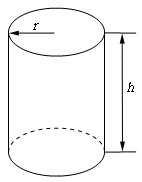
\includegraphics[width=0.2\textwidth]{figures/cylinder.png}
\caption{Graphical representation of the \emph{can} minimization example.}
\label{fig:cylinder}
\end{figure}

Clearly to minimize the costs, the company needs to reduce the amount of aluminum used in the production, consequently the can surface. 

So in this case the objective function, computes the sum of the lateral surface plus twice the base surface (i.e. the area of a cylinder).

\begin{equation} 
S = 2\pi rh + 2\pi r^2 
\label{eq:can_surface}
\end{equation}
On the other hand the can volume is fixed to 33~cl or 330~\(\mathrm{cm}^3\) and this allows to simplify the previous equation by removing \(h\)

\begin{equation*} 
V = \pi r^2 h = 330\quad\implies h = \cfrac{330}{\pi r^2}
\end{equation*}
Replacing $h$ in Eq.~\ref{eq:can_surface} 

\begin{equation}
S = 2\pi rh + 2\cdot(\pi r^2) = \cfrac{2\cdot 330}{r} + 2\cdot(\pi r^2)
\end{equation}
This is the objective function, and the parameter set (just one parameter in this case) is represented by \texttt{x[0]} which is the can radius in cm. It is convenient to use a \texttt{list} (or a \texttt{numpy.array}) also in this simple case since it can be generalized to more complex problems with a larger number of parameters to minimize. 

\begin{ipython}
from math import pi

def obj_func(x):
    return 2*330/x[0] + 2*pi*x[0]**2
\end{ipython}
\noindent
Set the limits to our unknown variable and its initial value:

\begin{ipython}
x0 = [1]
bounds = [(0.01, 100)]
\end{ipython}
\noindent
Finally run the minimization:

\begin{ipython}
from scipy.optimize import minimize

r = minimize(obj_func, x0, bounds=bounds)
print (r)
\end{ipython}
\begin{ioutput}
      fun: 264.356810914805
 hess_inv: <1x1 LbfgsInvHessProduct with dtype=float64>
      jac: array([5.68434189e-06])
  message: b'CONVERGENCE: NORM_OF_PROJECTED_GRADIENT_<=_PGTOL'
     nfev: 24
      nit: 9
   status: 0
  success: True
        x: array([3.7449385])
\end{ioutput}
So to minimize production costs the company should produce cans with a radius of about 3.745~cm (or about 74~mm diameter).

\begin{curiosity}
It looks like Coke has done a similar calculation since the result is surprisingly close to that of a real can. 

From \href{	https://www.ball.com/eu/solutions/markets-capabilities/capabilities/beverage-cans/standard-range
}{here} seems that a real can has a 66.3~mm diameter, a little smaller than our but it is not surprising since the real can shape is more elaborated than a simple cylinder.
\end{curiosity}

\subsubsection{Example with Constraint}
\label{example-with-constraint}

We are going to fence a rectangular field. If we look at the field from above the cost of the vertical sides are \$10/m, the cost of the
bottom side is \$2/m and the cost of the top side is \$7/m. If we have a \$700 budget determine
the dimensions of the field that will maximize the enclosed area, see Fig.~\ref{fig:field}.

\begin{figure}[h]
\centering
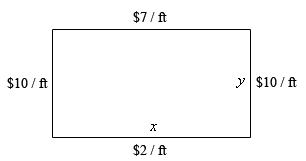
\includegraphics[width=0.4\textwidth]{figures/field.png}
\caption{Graphical representation of the \emph{field} minimization example.}
\label{fig:field}
\end{figure}

In this example there are two differences with respect to the previous:

\begin{itemize}
\tightlist
\item
  we want to \emph{maximize} a quantity (not minimize);
\item
  there is a constraint (we have a limited budget).
\end{itemize}

So let's repeat the steps as before. The objective is to maximize the enclosed area \(A\) but we have a problem since our algorithm can only minimize functions. To overcome this issue the objective function can be defined to return the quantity \(-A\), so that minimizing its value, the real objective, $A$, is maximized. 
Define length and width of the field respectively as \(\tt{x[0]}\) and \(\tt{x[1]}\) (items of the \texttt{list} \texttt{x}):

\begin{ipython}
def obj_func(x):
    return -x[0]*x[1]
\end{ipython}
Then we can set the boundaries for length and width, their initial values (1~m each) and the other needed parameters:

\begin{ipython}
x0 = [1, 1]
bounds = [(0.01, 100) for _ in range(len(x0))]
budget = 700
side_cost = 10
up_cost = 2
down_cost = 7
\end{ipython}

Finally we have to impose the budget constraint. This is done by defining a function that computes the fence cost and compare it to the total budget. 
The constraint is passed to the minimizer as a dictionary (or a list  of dictionaries if there are more) which has three keys: \(\tt{type}\), in this case set to \texttt{'eq'} (like equality, since we want to spend all of our available money so the fence has to cost exactly \$700), \texttt{'fun'} which defines the constraint function and \texttt{'args'} which is optional and is set to a tuple whose items are the possible parameters for the constraint function (see Section~\ref{sec:kwargs_args}).

The constraint is then defined as

\begin{equation*}
\begin{cases}
\mathrm{fence~cost} = l\cdot\mathrm{side\_cost} + l\cdot\mathrm{side\_cost} + w\cdot\mathrm{up\_cost} + w\cdot\mathrm{down\_cost}\\
\mathrm{budget} - \mathrm{fence~cost} = \mathrm{budget} - 2\cdot l\cdot\mathrm{side\_cost} - w\cdot(\mathrm{up\_cost} + \mathrm{down\_cost}) = 0
\end{cases}
\end{equation*}

\begin{ipython}
def cons(x, budget, up_cost, down_cost, side_cost):
    return budget - 2*x[0]*side_cost - x[1]*(up_cost + down_cost)

constraints = {'type':'eq', 'fun':cons,
               'args':(budget, up_cost, down_cost, side_cost)}
\end{ipython}

Now we can call the minimizer.

\begin{ipython}
r = minimize(obj_func, x0, bounds=bounds, constraints=constraints)
print (r)
\end{ipython}
\begin{ioutput}
    fun: -680.5555555555482
    jac: array([-38.88889313, -17.5       ])
message: 'Optimization terminated successfully'
   nfev: 12
    nit: 4  
   njev: 4
 status: 0
success: True
      x: array([17.49999818, 38.88889293])
\end{ioutput}

The field will come out 17.5~m long and 38.9~m wide for a total field area of 680.5~$\textrm{m}^2$.

\subsection{Local Minima}
Minimization problems can be very nasty.
For example when the objective function has local minima the choice of the initial value of the parameters can be critical. 
Assume we would like to minimize an objective function like 

\[
f(x) = \cfrac{\mathrm{cos}(3\pi x)}{x}
\]
This function is plotted in Fig.~\ref{fig:local_minima} in the range $[0, 2]$, and clearly it has many minima. 

\begin{figure}[htb]
	\centering
	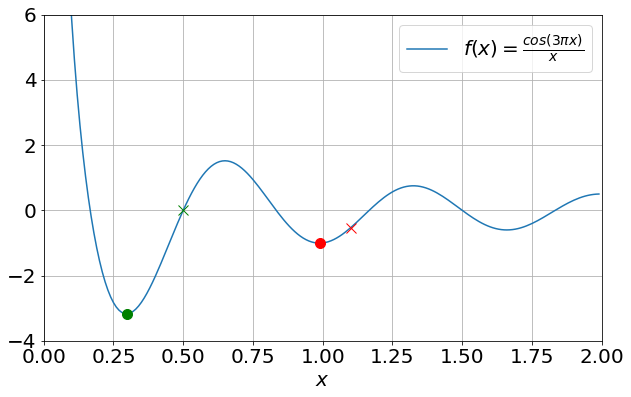
\includegraphics[width=0.7\textwidth]{figures/local_minima}
	\caption{Plot of an example function with many local minima. The red points highlights initial value and minimum found in a \emph{bad} minimization, green points for a good minimization.}
	\label{fig:local_minima}
\end{figure}
Let's try to find a minimum setting the initial value to $x=1.1$.
\begin{ipython}
x0 = [1.1]
bounds = [(0.01, 20)]
r = minimize(func, x0, bounds=bounds)

print (r)
\end{ipython}
\begin{ioutput}
     fun: array([-1.00569871])
hess_inv: <1x1 LbfgsInvHessProduct with dtype=float64>
     jac: array([-4.4408921e-07])
 message: b'CONVERGENCE: NORM_OF_PROJECTED_GRADIENT_<=_PGTOL'
    nfev: 16
     nit: 5
  status: 0
 success: True
       x: array([0.98865633])
\end{ioutput}
The minimization worked perfectly and we found $x=0.98865633$ (i.e. the red point in Fig.~\ref{fig:local_minima}) but this is not the absolute minimum we were expecting to find. The problem arise since the algorithm, following the derivative direction, has got stuck in a local minimum without any possibility to jump out from the well.

If we repeat the minimization using as initial value $0.5$ instead
\begin{ipython}
x0 = [0.5]
bounds = [(0.01, 20)]
r = minimize(func, x0, bounds=bounds)

print (r)
\end{ipython}
\begin{ioutput}
     fun: array([-3.17151711])
hess_inv: <1x1 LbfgsInvHessProduct with dtype=float64>
     jac: array([9.76996262e-07])
 message: b'CONVERGENCE: NORM_OF_PROJECTED_GRADIENT_<=_PGTOL'
    nfev: 16
     nit: 5
  status: 0
 success: True
       x: array([0.29691798])
\end{ioutput}
Now clearly the algorithm found the absolute minimum in $x=0.29691798$ (i.e. the green point in Fig.~\ref{fig:local_minima}) because there was no chance to find a local minimum during the iterations.

This is just an example of what could happen when minimizing a function. When dealing with complicated cases it is possible to make a \emph{scan} of the objective function to try to approximately determine where the global minimum is and choose suitable initial values of the guess parameters.
However there shouldn't be such an issue in the application of the bootstrap algorithm since the function that is minimized is a sum of squared terms which has no local minimum, just a global minimum (i.e. it is a hyper-parabola).

\subsection{Back to Bootstrapping}
\label{ois-example}

Here the problem consists of finding the discount curve $\mathcal{C}$ such that it prices as much correctly as possible each OIS by minimizing the sum of the squared NPVs (our $f_i$):

\begin{equation}
	\mathrm{min}_{\mathcal{C}} \Big\{\sum_{i=1}^{n}\mathrm{NPV}(\mathrm{OIS}_i, \mathcal{C})^2\Big\}
\end{equation}

Remember we are assuming that the market quotes represent the OIS \emph{fair} prices, so their NPV's should be close to 0.

The previous equation is the objective function to implement, and the algorithm will adjust the unknown discount factors of $\mathcal{C}$ to reach the minimum.

In the previous examples though, the number of minimization parameters (i.e. the degrees of freedom of the problem) was clear:
\begin{itemize}
\item 1 for the can example, the can radius;
\item 2 for the fence problem, width and height of the field.
\end{itemize}

A discount curve is characterized by pillar dates ($\mathbf{d}$) and discount factors ($\mathbf{x}$), but we haven't yet identified a constraint on how many points the curve is made of (too many points or too few may prevent us from finding the solution).
\textbf{In practice, it makes sense to choose the number of degrees of freedom to match the number of market quotes.} In particular it is wise to choose the pillar dates of the discount curve equal to the set of the swap expiry dates.

\begin{equation}
 F= \mathrm{min}_{\mathbf{x}} \Big\{\sum_{i=1}^{N}\mathrm{NPV}^2(\mathrm{OIS}_i, \mathcal{C}(\mathbf{d}, \mathbf{x}))\Big\}\qquad (f_i^2 = \mathrm{NPV}^2(\mathrm{OIS}_i, \mathcal{C}(\mathbf{d}, \mathbf{x})))
\end{equation}
which is the final version of our optimization problem (i.e. finding the minimum of the above expression as a function of $\mathbf{x}$).

First the swaps has to be created according to all the available market quotes

\begin{ipython}
from finmarkets import generate_dates
from datetime import date

observation_date = date.today()
pillar_dates = [observation_date]
swaps = []

for i in range(len(mq)):
    swap = OvernightIndexSwap(1e6,
             generate_dates(observation_date,
                            mq.loc[i, 'months']),
             0.01 * mq.loc[i, 'quote'])
    swaps.append(swap)
	pillar_dates.append(swap.payment_dates[-1])

# this last command doesn't matter if swap are originally
# sorted by maturity	
pillar_dates = sorted(pillar_dates)
\end{ipython}

Then implement step by step the bootstrapping as described in Section~\ref{sec:bootstrap_as_minimization}

\begin{itemize}
\tightlist
\item
  define the objective function: the sum of the squared NPVs of the OIS (today's discount factor is fixed to 1 so it may not be included in the minimization parameters, hence it is added in the function definition). Note that any objective function can have constant additional parameters beside those used in the minimization, the convention assumes that the first parameter of the function must be those to minimize. 

\begin{ipython}
import numpy as np

def objective_function(x, obs_date, pillars):
    x = np.insert(x, 0, 1)
    curve = DiscountCurve(pillars, x)
    sum_sq = 0.0
    for swap in swaps:
        sum_sq += swap.npv(curve) ** 2
    return sum_sq
\end{ipython}

\item
  set the initial value of the discount factors (\(x_i^0\)) to 1 with a
  range of variability \([ 0.01, 10]\), (again today's discount factor is not considered 
  in the list, see \texttt{insert} command)

\begin{ipython}
x0 = [1.0 for i in range(len(pillar_dates)-1)]
bounds = [(0.01, 10.0) for i in range(len(pillar_dates)-1)]
\end{ipython}

\item
  finally we can launch the minimizer to find the discount factors
  (\(\mathbf{x}\))

\begin{ipython}
result = minimize(objective_function, x0, bounds=bounds,
                  args=(observation_date, pillar_dates))

print (result)
\end{ipython}
\begin{ioutput}
      fun: 0.0006561234813731959
 hess_inv: <30x30 LbfgsInvHessProduct with dtype=float64>
      jac: array([-1.46749218, -1.52880351, -1.58043371, -1.62444368,
                  -1.65793781, -1.68430928, -1.69973037, -1.70611237, 
                  -1.70035125, -1.68091034, -1.64422388, -6.24051456,  
                   2.15976419,  1.88313032,  1.73861385, -1.39376647,  
                   3.25043542,  6.29526861,  4.68446978,  0.59831059,
                  -2.50678569, -2.87296531, -0.35746643,  3.87250114,  
                   8.63671196, -1.6629543 ,  4.92871632,  2.83505097, 
                  -1.31891876, -1.77479162])
  message: b'CONVERGENCE: REL_REDUCTION_OF_F_<=_FACTR*EPSMCH'
     nfev: 496
      nit: 9
   status: 0
  success: True
  x: array([1.00029175, 1.00058832, 1.00088044, 1.00118752,
  1.00148972, 1.00176787, 1.00207128, 1.00236508, 1.00266885,
  1.002963  , 1.0032578 , 1.00356136, 1.00444991, 1.00529984,
  1.00614269, 1.00693073, 1.00907045, 1.00931993, 1.00710124,
  1.00189872, 0.99379275, 0.98332974, 0.97101001, 0.95723162,
  0.94267503, 0.9277256 , 0.8831291 , 0.81781096, 0.76554623,
  0.71988353, 0.64350526, 0.5928188 , 0.54546435])
\end{ioutput}
\end{itemize}

Printing the result gives us the a lot of information about the minimisation just performed, the most useful are:
\begin{itemize}
\item \texttt{func}: the objective function value at the last iteration;
\item \texttt{message}: the summary message (if it is \texttt{CONVERGENCE} is almost always OK);
\item \texttt{success}: the name is self explanatory;
\item \texttt{x}: the vector of unknown parameters that have been optimised.
\end{itemize}

Another useful check to perform in order to understand if everything went fine, is the comparison of the objective function value at the beginning and at the end of the minimization.

\begin{ipython}
print ("Initial objective function value ", objective_function(x0))
print ("Final objective function value ", objective_function(result.x))
\end{ipython}
\begin{ioutput}
Initial objective function value  1399018851176.301
Final objective function value  0.0006561234813731959
\end{ioutput}
The objective function at the end of the minimisation is not exactly 0 (and rarely it will be) but its value is small enough for us to be satisfied, the initial value was around $10^{11}$ and now it is $10^{-4}$ so 15 orders of magnitude smaller. This means that with the derived discount curve the NPV's of our OIS won't be identically 0 but so small that can be regarded as they would.

It can be very useful to also look at some diagnostic plots to check if the minimization was successful. Figure~\ref{fig:minimization_diagnostic} reports on the left the objective function value as a function of discount factor $(x_0)$; clearly we have found a minimum (the orange point represent $x_0$ value at the end of the minimization). On the right instead, the value of the objective function at each iteration is shown, its value is decreasing dramatically (notice that the $y$ axis is drawn in log scale).

\begin{figure}[htb]
	\centering
	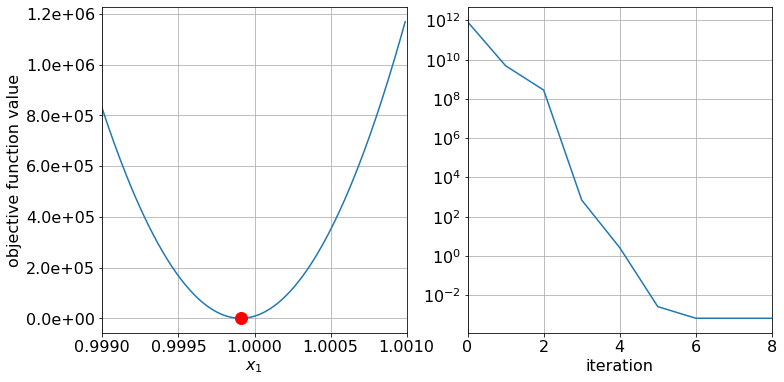
\includegraphics[width=0.9\linewidth]{figures/obj_func_diagnostic}
	\caption{Diagnostic plots for the minimization algorithm. On the left the objective function value as a function of the discount factor $x_1$ (the red point represent $x_0$ value at the end of the minimization), on the right the objective function value as a function of the iteration number.}
	\label{fig:minimization_diagnostic}
\end{figure}

Finally we can create the discount curve implied by the market quotes of our swaps (see Fig.~\ref{fig:discount_curve}) and try to compute some implied rates (remember to add back the first discount factor to the vector of parameters).

\begin{ipython}
from math import log
from dateutil.relativedelta import relativedelta

dfs = np.insert(result.x, 0, 1)
curve = DiscountCurve(pillar_dates, dfs)
d = observation_date + relativedelta(years=40)

print ("40y df: {:.3f}".format(curve.df(d)))
print ("40y rate: {:.4f}".format(-log(curve.df(d)) / 20))
\end{ipython}
\begin{ioutput}
40y df: 0.643
40y rate: 0.0110
\end{ioutput}

\begin{figure}[htb]
	\centering
	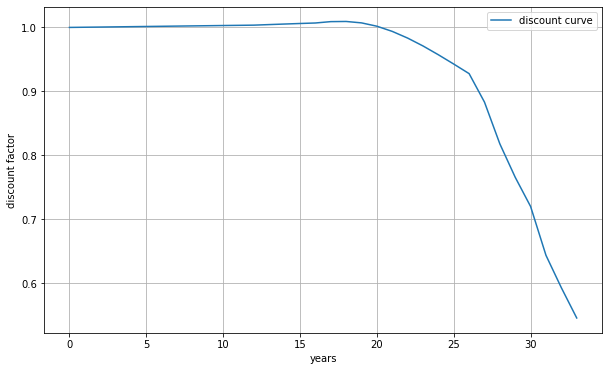
\includegraphics[width=0.7\textwidth]{figures/example_discount_curve}
	\caption{Plot of the discount curve implied by Overnight Index Swap market quotes.}
	\label{fig:discount_curve}
\end{figure}

\section{Discount Factors with Pseudo-inverse}
An alternative procedure to derive discount factors involves matrix inversion and in some special cases the usage of the \emph{pseudoinverse} described in Section~\ref{sec:the-moore-penrose-pseudoinverse}.Details on this algorithm can be found in~\cite{bib:boostrap_pseudoinv}.

Consider a set of $n$ financial instruments (e.g. bonds, futures, swaps, \ldots). The price of such instruments is connected to the discount factors by the following relationship

\begin{equation}
P_i = \sum_{j=0}^{m} C_{i,j} d_j
\label{eq:discounted_cashflows}
\end{equation}
where $P_i$ is the market quote of the $i^{th}$ product, $C_{i,j}$ is the $j^{th}$ cash-flow of the $i^{th}$ product and $d_j$ is the discount factor relative to period $(t_0, t_j)$.
Eq.~\ref{eq:discounted_cashflows} can be written in matrix form

\begin{equation}
\boldsymbol{P} = [C]\boldsymbol{d}
\label{eq:discount_matrix}
\end{equation}
and now $P$ and $d$ are column vectors while $[C]$ is a $n \times m$ matrix where each row element is a cash-flow associated to the row product.

Recalling Section~\ref{solving-systems-of-equations-using-matrix-inverses}, Eq.~\ref{eq:discount_matrix} represents a system of equations which can be solved to determine the unknown $\boldsymbol{d}$.
The sought solution is 
\begin{equation}
\boldsymbol{d} = [C^{-1}] \boldsymbol{P}
\end{equation} 
If matrix $[C]$ is not invertible (i.e. the system of equations is under-determined) $[C^{-1}]$ can be replaced by the optimal approximation $[C^+]$ (i.e. the pseudo-inverse). 

To illustrate the algorithm let's consider again the previous example with five coupon bearing bonds (coupon of 4\%, 5\%, 6\%, 7\% and 8\% respectively) with maturities ranging from 1 to 5 years, each having a value of \euro{100} and traded at par. In this case we have
\begin{equation*}
\boldsymbol{P} = 
\begin{bmatrix}
100 \\
100 \\
100 \\
100 \\
100 
\end{bmatrix}; \quad
[C] = 
\begin{bmatrix}
104 & 0 & 0 & 0 & 0 \\
5 & 105 & 0 & 0 & 0 \\
6 & 6 & 106 & 0 & 0 \\
7 & 7 & 7 & 107 & 0 \\
8 & 8 & 8 & 8 & 108
\end{bmatrix}; \quad \boldsymbol{d} =
\begin{bmatrix}
d_1 \\
d_2 \\
d_3 \\
d_4 \\
d_5 
\end{bmatrix}
\end{equation*}
The \texttt{python} implementation to determine the solution is given in the snippet below. The code use by default the pseudo-inverse since if $[C]$ is invertible holds $[C^+] = [C^{-1}]$. 
\begin{ipython}
import numpy as np

C = np.array([[104, 0, 0, 0, 0],
              [5, 105, 0, 0, 0],
              [6, 6, 106, 0, 0],
              [7, 7, 7, 107, 0],
              [8, 8, 8, 8, 108]])
P = np.array([100, 100, 100, 100, 100])

Cinv = np.linalg.inv(C)
d = Cinv.dot(P.T)
print (d)
\end{ipython}
\begin{ioutput}
[0.96153846 0.90659341 0.83765291 0.75756548 0.66938146]	
\end{ioutput}
To determine the corresponding yields just use \texttt{brentq} to solve $1/(1+y_n)^{n}$
\begin{ipython}
from scipy.optimize import brentq

def rate(x, d, tau):
    return d - 1/(1+x)**tau

for i in range(5):
    print ("yield y{}: {:.4f}".format(i+1, brentq(rate, 0, 1, args=(d[i], i+1))))
\end{ipython}
\begin{ioutput}
yield y1: 0.0400
yield y2: 0.0503
yield y3: 0.0608
yield y4: 0.0719
yield y5: 0.0836
\end{ioutput}
which matches those in Table~\ref{tab:rates}.

In this simple example just bonds were considered but clearly the method can be extended also to other instruments when creating the cash-flow matrix $[C]$.

\section*{Exercises}
\begin{question}
Consider two 5\% coupon paying bonds (par value of \euro{100}) with the clean market prices of \euro{99.50} and \euro{98.30} and having maturities of 6 months and 1 year respectively.
Determine the spot rate for the 6-month and 1-year bond.  
\end{question}

\begin{solution}
At the end of 6 months the first bond will pay a coupon of \euro{2.5} (= \euro{100} * 5\%/ 2) plus the principal amount (= €100) which sums up to 102.50. To
determine the 6M spot rate we can write the following equation, :

\[ \cfrac{102.5}{(1 + S_{6M}/2)} = 99.5\qquad\Rightarrow\qquad S_{6M} = 2 \cdot \Big( \cfrac{102.5}{99.5} - 1 \Big) =  6.03 \%\]

At the end of another 6 months the second bond will pay a coupon of €2.5
(= €100 * 5\% / 2) plus the principal amount (= €100) which sums up to
€102.50. The bond is trading at €98.30, therefore, the 1-year spot rate
\(S_{1y}\) can be calculated using \(S_{6M}\) as,

\[ \cfrac{2.5}{(1+S_{6M}/2)} + \cfrac{102.5}{(1 + S_{1y}/2)^{2}} = 98.30 \]

\[ \cfrac{102.5}{(1 + S_{1y}/2)^{2}} = 98.30 - \cfrac{2.5}{(1+0.03015)} \]

\[ (2 + S_{1y})^{2} = \cfrac{4\cdot102.5}{98.87317} = 4.276428 \]

\[ S_{1y}^{2} + 4\cdot S_{1y} - 0.276428 = 0 \]

\[ S_{1y} = -2 \pm \sqrt{4 + 0.276428} =\begin{cases}\text{\sout{-4.06795}} \\ 6.80\%\end{cases} \]

\end{solution}

\begin{question}
A small petroleum company owns two refineries. Refinery 1 costs \$20,000 per day to operate, and it can produce 400 barrels of high-grade oil, 300 barrels of medium-grade oil, and 200 barrels of low-grade oil each day. Refinery 2 is newer and more modern. It costs \$25,000 per day to operate, and it can produce 300 barrels of high-grade oil, 400 barrels of medium-grade oil, and 500 barrels of low-grade oil each day.
The company has orders totaling 25,000 barrels of high-grade oil, 27,000 barrels of medium-grade oil, and 30,000 barrels of low-grade oil. How many days should it run each refinery to minimize its costs and still refine enough oil to meet its orders?

\noindent\textbf{Hint:} you need to identify the unknown quantities (working days for each refinery) and set the constraints on the production of barrels. The objective is to minimize the costs. If you have multiple constraints you can define a list of dictionaries (one for constraint). Furthermore in this case the constraint is not \emph{equal to} but rather \emph{greater than} so you have to set \texttt{ineq} type.
\end{question}

\cprotEnv\begin{solution}
Let's implement the usual steps for a minimization. In this case our unknown are \texttt{x[0]} and \texttt{x[1]} the working days for each refinery. Then define the objective function with the production costs and three more functions, one for each oil-grade for the constraints.

\begin{ipython}
from scipy.optimize import minimize

def of(x):
    return 20000*x[0] + 25000*x[1]

def cons1(x):
    return 400*x[0] + 300*x[1] - 25000

def cons2(x):
    return 300*x[0] + 400*x[1] - 27000

def cons3(x):
    return 200*x[0] + 500*x[1] - 30000

cons = [{"type":"ineq", "fun":cons1},
        {"type":"ineq", "fun":cons2},
        {"type":"ineq", "fun":cons3}]
\end{ipython}
Set limits and initial values and run the minimizer.
\begin{ipython}
x0 = [10, 10]
bounds = [(0, 100) for _ in range(len(x0))]
r = minimize(of, x0, bounds=bounds, constraints=cons)
print (r)
\end{ipython}
\begin{ioutput}
     fun: 1750002.070622686
     jac: array([20000., 25000.])
 message: 'Optimization terminated successfully.'
    nfev: 8
     nit: 6
    njev: 2
  status: 0
 success: True
       x: array([25.00004033, 50.00005056])
\end{ioutput}    
So refinery 1 should work 25 days while refinery 2 50 days to minimize the production costs to 1750000 M (see objective function value in the minimization report).
\end{solution}

\begin{question}
Read the OIS market data from \href{https://drive.google.com/file/d/1LCEDmheKqwPXFpJ25hFz32QI5im2UJO1/view?usp=sharing}{\texttt{ois\_data.xlsx}} and, using the \texttt{OvernightIndexSwap} class,construct the corresponding swaps.
\end{question}

\cprotEnv\begin{solution}

\begin{ipython}
import pandas, datetime
from finmarkets import OvernightIndexSwap, generate_swap_dates

observation_date = datetime.date.today()
df = pandas.read_excel('ois_data.xlsx')

market_quotes = {}
for i in range(len(df)):
    key = df.loc[i, 'months']
    value = df.loc[i, 'quote']
    market_quotes[key] = value

swaps = []
for months, rate in market_quotes.items():
    swap = OvernightIndexSwap(1e6,
        generate_swap_dates(observation_date, months),
        0.01 * rate)

swaps.append(swap)
\end{ipython}
\end{solution}

\begin{question}
From the \texttt{OvernightIndexSwap} created in the previous example derive a discount curve using the bootstrap method.
\end{question}

\cprotEnv\begin{solution}
We have just created some swaps from the market quotes in the previous exercise, so now we can just create a list with the pillar dates.

\begin{ipython}
observation_date = date(2019, 10, 23)
pillar_dates = [observation_date]

for swap in swaps:
    pillar_dates.append(swap.payment_dates[-1])

# this shouldn't be necessary if the original
# list of market quotes is sorted
pillar_dates = sorted(pillar_dates)
\end{ipython}
Define the objective function: the sum of the squared NPVs of the OIS.
\begin{ipython}
def objective_function(x):
    curve = DiscountCurve(observation_date,
        pillar_dates, x)

    sum_sq = 0.0
    for swap in swaps:
        sum_sq += swap.npv(curve) ** 2
    return sum_sq
\end{ipython}
Set the initial value of the discount factors (\(x_i\)) to 1 with a range of variability \([ 0.01, 10]\), in addition the first element of the list, today's discount factor, will be fixed to 1 (variability \([1, 1]\)).

\begin{ipython}
x0 = [1.0 for i in range(len(pillar_dates))]

bounds = [(0.01, 10.0) for i in range(len(pillar_dates))]
bounds[0] = (1.0, 1.0)
\end{ipython}
Finally launch the minimizer to find the discount factors (\(\mathbf{x}\)).

\begin{ipython}
from scipy.optimize import minimize

result = minimize(objective_function, x0, bounds=bounds)
print (result)
\end{ipython}
\begin{ioutput}
     fun: 0.000819919032900304
hess_inv: <34x34 LbfgsInvHessProduct with dtype=float64>
     jac: array([ 6.58948735e+05, -1.58720803e+01, -6.53143264e+01, 
                 -1.03323232e+02, -1.26050260e+02, -1.31748898e+02, 
                 -1.20374599e+02, -9.15399651e+01, -4.24363322e+01,  
                  2.44903182e+01,  1.14345243e+02,  2.22002243e+02,
                 -3.72021700e+00,  4.21398633e+01,  4.21787852e+01,  
                  4.22369487e+01,  4.23327026e+01,  4.31814758e+01,  
                  4.44924460e+01,  4.62078978e+01,  4.82906823e+01, 
                  -3.69972738e+00,-1.42454702e+00,  7.53771932e-01,
                  2.79741018e+00,  4.62896699e+00,  6.24844054e+00,  
                  9.93101553e+00,  1.31122434e+01,  1.42880909e+01,  
                  1.48279215e+01,  1.50787019e+01,  1.43267935e+01,  
                  1.38451324e+01])
 message: b'CONVERGENCE: REL\_REDUCTION\_OF\_F\_<=\_FACTR*EPSMCH'
    nfev: 840
     nit: 7
  status: 0
 success: True
       x: array([1.        , 1.00030147, 1.00058831, 1.00089012, 1.00119726,
                 1.00147996, 1.00178743, 1.00208107, 1.00238467, 1.00267865,
                 1.00298261, 1.00327737, 1.00357104, 1.00357104, 1.00355063,
                 1.00352002, 1.00346901, 1.00302007, 1.00232627, 1.00141821,
                 1.00031629, 0.99911234, 0.99790839, 0.99675545, 0.99567393,
                 0.99470465, 0.9938476 , 0.99189884, 0.99021534, 0.98959296,
                 0.98930728, 0.98917464, 0.98957256, 0.98982763])
\end{ioutput}
\end{solution}

%\begin{question}
%Take the \texttt{OvernightIndexSwap} class from \texttt{finmarkets} module and add a new method called \texttt{fair\_value\_strike} which takes a discount curve object and returns the fixed rate which would make the OIS with zero NPV.
%
%\noindent\textbf{Hint:} first take the formulas for the NPV of the fixed and floating legs, put one equal to the other and solve for $K$.
%\end{question}
%
%\cprotEnv\begin{solution}
%As the hint suggested the two NPV equations are compared:
%
%\[\mathrm{NPV}_{\mathrm{fix}} = NK \sum_{i=1}^{n}D(d_{i})\cfrac{d_i - d_{i-1}}{360}\]
%
%\[\mathrm{NPV}_{\mathrm{float}} = N \cdot [D(d_0) - D(d_n)]\]
%
%\[K \sum_{i=1}^{n}D(d_{i})\cfrac{d_i - d_{i-1}}{360} = [D(d_0) - D(d_n)]\]
%
%\[K = \cfrac{[D(d_0) - D(d_n)]}{\sum_{i=1}^{n}D(d_{i})\cfrac{d_i - d_{i-1}}{360}}\]
%Now in \texttt{python}:
%
%\begin{ipython}
%class OverNightIndexSwap:
%    ...
%    def fair_value_strike(self, discount_curve):
%        den = 0
%        for i in range(1, len(self.payment_dates)):
%            start_date = self.payment_dates[i-1]
%            end_date = self.payment_dates[i]
%            tau = (end_date - start_date).days / 360
%            df = discount_curve.df(end_date)
%            den += df * tau
%            num = (discount_curve.df(self.payment_dates[0]) -
%                discount_curve.df(self.payment_dates[-1]))
%        return num/den
%\end{ipython}
%Finally add this method to the class implementation in \texttt{finmarkets.py}.
%\end{solution}


\begin{thebibliography}{9}
\bibitem{bib:default_from_bond} J. C. Hull, \emph{Options, Futures and Other Derivatives, 7th Ed.}, Swaps (Ch. 7), Pearson Prentice Hall, 2009
\bibitem{bib:bootsrap} \href{https://financetrain.com/bootstrapping-spot-rate-curve-zero-curve}{\emph{Bootstrapping Spot Rate Curve}} [Online]
\bibitem{bib:boostrap_pseudoinv} D. Filipovic, S. Willems, \emph{Exact Smooth Term-Structure Estimation}, arXiv: 1606.03899, February 12, 2018
\end{thebibliography}
